%Đây là template dùng cho đề cương đề tài tốt nghiệp
%Khoa Công nghệ Thông tin
%Trường Đại học Khoa học Tự nhiên, ĐHQG-HCM

%Liên hệ về mẫu LaTEX này: Thầy Bùi Huy Thông (bhthong@fit.hcmus.edu.vn)

\documentclass{article}[14pt]
\usepackage[utf8]{vietnam}
\usepackage{enumerate}
\usepackage{enumitem}
\usepackage{multicol}
\usepackage{listings}
\usepackage[left=2cm,right=2cm,top=2.5cm,bottom=2.5cm]{geometry}
\usepackage{verbatim}
\usepackage{graphicx}
\usepackage{url}
\usepackage{fancyhdr}
\usepackage{fancybox,framed}
\linespread{1.3}
\usepackage{lastpage}
\usepackage{floatrow}
\usepackage{floatrow}
\usepackage[utf8]{inputenc}
\usepackage{array}
\usepackage{longtable}
\usepackage{geometry}
\geometry{a4paper, margin=1in}
\pagenumbering{arabic}
%\pagestyle{fancy}
\newfloatcommand{capbtabbox}{table}[][\FBwidth]
\usepackage{caption}
\captionsetup[figure]{font=large} 
\usepackage{blindtext}
\usepackage{titlesec}
\usepackage[nottoc]{tocbibind}

\titleformat*{\section}{\LARGE\bfseries}
\titleformat*{\subsection}{\Large\bfseries}
\titleformat*{\subsubsection}{\large\bfseries}
%\addbibresource{ref.bib}


\begin{document}
    \begin{figure}[h]
        \begin{floatrow}
        \ffigbox{
\includegraphics[scale = .4]{logo.png}}  
        {%
    
        }
        \capbtabbox{
            \begin{tabular}{l}
            \multicolumn{1}{c}{\textbf{\begin{tabular}[c]{@{}c@{}}TRƯỜNG ĐẠI HỌC KHOA HỌC TỰ NHIÊN\\KHOA CÔNG NGHỆ THÔNG TIN\end{tabular}}} \\ \\ \\
            \end{tabular}
        }
        {%
    
        }
        \end{floatrow}
    \end{figure}
    
    \begin{center}
        
        %Xác định loại đề tài tốt nghiệp tương ứng: Khóa luận, Thực tập, Đồ án
        \textbf{\Large ĐỀ CƯƠNG LUẬN VĂN \\  TỐT NGHIỆP} \\ 
    \end{center}
    
    %\vspace{.5cm}
    
    \begin{center}
    %Tên đề tài phải VIẾT HOA
        
        \textbf{\huge Hệ quản trị cơ sở dữ liệu quan hệ phân tán hỗ trợ xử lý dữ liệu lớn trực tuyến } 
        \\
        
    %Tên đề tài bằng tiếng Anh (nếu có)
    \vspace{.5cm}
        \textit{\textbf{\Large (Distributed Relational Database Management System Supporting Online Big Data Processing  )}}
    \end{center}
    
    \vspace{.5cm}
    
    \Large
    \section{THÔNG TIN CHUNG}
    \begin{itemize}[label = {}]
        
        \item \textbf{Người hướng dẫn:} 
        %Thể hiện dạng: <Chức danh> <Họ và tên> (<Đơn vị công tác>)
        \begin{itemize}
            \item TS. Ngô Huy Biên (Khoa Công nghệ Thông tin)
        \end{itemize}{}
    
        
        \item \textbf{Học viên thực hiện:}
        
        %Thể hiện dạng: <Họ và tên sinh viên> (MSSV: )
        \begin{itemize}
        
            \item Trần Hữu Nghĩa (MSSV: 21C12005) 
           
        \end{itemize}

       %Chọn loại thích hợp
        \item \textbf{Mã số ngành:} 8480104
        
        \item \textbf{Thời gian thực hiện:} Từ \textit{06/2023} đến \textit{12/2023}
        
        
    \end{itemize}
    
    \pagebreak 
    
    \section{NỘI DUNG THỰC HIỆN}
    {

    %Mỗi mục dưới đây phải viết ít nhất là 5 câu mô tả/giới thiệu.
    
    \subsection{Giới thiệu tổng quan }
    
Các hệ thống cơ sở dữ liệu quan hệ truyền thống gặp khó khăn trong việc xử lý dữ liệu lớn khi thực hiện các hoạt động OLAP (Online Analytical Processing) do khả năng mở rộng hạn chế và hiệu suất truy vấn không tốt. Việc mở rộng hệ thống cơ sở dữ liệu để đáp ứng nhu cầu tăng lên của người dùng và dữ liệu có thể là một thách thức lớn. Một số hệ thống không hỗ trợ mở rộng theo cả hai chiều (scale-up và scale-out), điều này có thể hạn chế khả năng của tổ chức để mở rộng hệ thống của họ khi cần dẫn đến thời gian phản hồi truy vấn chậm và lãng phí tài nguyên (như bộ vi xử lý, bộ nhớ).


Apache Hive\cite{aluko2019big}, một hệ thống dữ liệu lớn phân tán dựa trên Hadoop, được thiết kế để xử lý và phân tích dữ liệu lớn bằng ngôn ngữ truy vấn giống SQL (HiveQL). Hive không phải là một hệ thống cơ sở dữ liệu thời gian thực, mà chủ yếu tập trung vào việc cung cấp khả năng phân tích dữ liệu lớn với độ trễ cao hơn. Hive sử dụng Hadoop MapReduce để thực hiện các truy vấn và chạy trên HDFS (Hadoop Distributed File System), cho phép phân tán và lưu trữ dữ liệu trên nhiều máy chủ. Tuy nhiên, Hive mang đến một số hạn chế. Độ trễ cao trong việc xử lý dữ liệu, khả năng tối ưu hóa truy vấn không mạnh mẽ, và dù hoạt động tốt trên hệ thống phân tán.

Tiếp theo là Spark SQL\cite{armbrust2015spark}, một thành phần của Apache Spark, đã khắc phục được một số nhược điểm của Hive. Spark SQL tận dụng công nghệ xử lý song song của Spark, giúp cải thiện hiệu suất và khả năng mở rộng, làm giảm thời gian truy vấn so với Hive. Nó sử dụng Catalyst Optimizer, một framework tối ưu hóa truy vấn mạnh mẽ, hỗ trợ xử lý dữ liệu cấu trúc và bán cấu trúc, và tương thích với Hive cũng như Hadoop, làm nó mở rộng khả năng tương tác với nhiều nguồn dữ liệu.

Bên cạnh Hive và Spark SQL, Greenplum\footnote{https://greenplum.org} cũng đóng một vai trò quan trọng trong lĩnh vực xử lý dữ liệu lớn. Greenplum là một hệ cơ sở dữ liệu Massively Parallel Processing (MPP) dựa trên PostgreSQL, một hệ thống quản lý cơ sở dữ liệu quan hệ mã nguồn mở. Nó được phát triển để xử lý khối lượng công việc dữ liệu quy mô lớn, dành riêng cho các ứng dụng phân tích, học máy và trí tuệ nhân tạo. Điều này giúp Greenplum cung cấp một số lợi ích mà Hive và SparkSQL không thể cung cấp, bao gồm khả năng quản lý và truy vấn hiệu quả petabytes dữ liệu theo cách phân tán.


Jason Arnold cùng các cộng sự đã đề xuất giải pháp có tên là “A High-Performance Distributed Relational Database System for Scalable OLAP Processing (HRDBMS)\cite{arnold2019hrdbms}. Nhận thấy những ưu điểm vượt trội và tiềm năng của giải pháp HRDBMS, luận văn này quyết định tập trung nghiên cứu và cài đặt giải pháp "tối ưu hóa truy vấn trên dữ liệu lớn" dựa trên các đề xuất của Jason Arnold.

HRDBMS với kiến trúc phân tán và khả năng xử lý song song, mang lại hiệu suất cao và linh hoạt khi thực hiện các truy vấn OLAP trên dữ liệu lớn. Nó cũng cho phép mở rộng khả năng xử lý truy vấn mà không làm giảm hiệu suất, một điều mà các hệ thống Hive, SparkSQL và Greenplum không thể đạt được hoàn toàn. Bằng việc tận dụng những khả năng này, luận văn hy vọng sẽ cung cấp một giải pháp tối ưu để tăng cường hiệu suất truy vấn trên dữ liệu lớn.

Mục tiêu chính của nghiên cứu này là khai thác, thử nghiệm và đánh giá hiệu năng của mã nguồn cùng các kỹ thuật trong hệ thống HRDBMS được trình bày trong công trình HRDBMS. Điều này nhằm xây dựng một hệ thống quản lý cơ sở dữ liệu hiệu năng cao, sánh ngang với các hệ thống MPP và có khả năng mở rộng tương đương với các nền tảng Big Data. Cụ thể như sau:

Thử nghiệm mã nguồn và áp dụng kỹ thuật: Tiến hành thử nghiệm mã nguồn và áp dụng các kỹ thuật của hệ thống HRDBMS, nhằm đánh giá hiệu quả và khả năng mở rộng của hệ thống trong thực tế.

Nghiên cứu hiệu năng trên mỗi node: Phân tích hiệu năng của hệ thống HRDBMS trên mỗi node, đánh giá sự phân tán và tính song song của hệ thống trong việc xử lý các truy vấn OLAP.

Đề xuất các phương pháp cải tiến và tối ưu hóa: Dựa trên kết quả thử nghiệm và đánh giá, đề xuất các phương pháp cải tiến và tối ưu hóa hệ thống HRDBMS, giúp nâng cao hiệu năng và khả năng mở rộng trong việc xử lý OLAP.
So sánh với các hệ thống MPP và nền tảng Big Data đối chiếu hiệu năng và khả năng mở rộng của hệ thống HRDBMS với các hệ thống MPP và nền tảng Big Data, nhằm xác định ưu nhược điểm của mỗi hệ thống trong việc xử lý dữ liệu lớn.

Qua việc thử nghiệm mã nguồn và áp dụng các kỹ thuật của hệ thống HRDBMS, đánh giá và nghiên cứu hiệu quả của các kỹ thuật này trong thực tế, đồng thời tìm hiểu về khả năng mở rộng của hệ thống và hiệu năng trên mỗi node. Mục tiêu cuối cùng là đề xuất các phương pháp cải tiến và tối ưu hóa hệ thống dựa trên những kết quả đạt được, nhằm mang lại giải pháp hiệu quả hơn cho việc xử lý OLAP trong các hệ thống cơ sở dữ liệu hiện đại.

\subsection{Mục đích nghiên cứu }

Nghiên cứu này tập trung vào việc phát triển một giải pháp tiên tiến để đương đầu với những thách thức tăng lên không ngừng từ việc quản lý và xử lý lượng dữ liệu lớn. Ngày nay, việc xử lý dữ liệu lớn đang trở thành một nhiệm vụ phức tạp, yêu cầu sự linh hoạt và hiệu suất tối ưu trong việc quản lý tài nguyên và truy vấn dữ liệu.

Vì vậy, mục tiêu chính của nghiên cứu này là xây dựng một hệ thống cơ sở dữ liệu phân tán, sử dụng các phương pháp tiên tiến. Nghiên cứu sẽ đánh giá tính khả thi và hiệu suất của hệ thống này trong việc xử lý và quản lý dữ liệu lớn.

Kết quả của nghiên cứu này sẽ mang lại những lợi ích thiết thực và giá trị đáng kể, đặc biệt cho những doanh nghiệp vừa và lớn trong lĩnh vực thương mại điện tử và bán lẻ và các cửa hàng bán lẻ vừa và nhỏ khác. Các tổ chức này hàng ngày phải tạo ra và xử lý một lượng lớn dữ liệu. Quản lý và tối ưu hóa quá trình này, họ cần một hệ thống quản lý dữ liệu hiệu quả và linh hoạt. Đáp ứng nhu cầu này, HRDBMS, trở thành lựa chọn tối ưu với các tính năng mạnh mẽ của mình.

HRDBMS, dựa trên mô hình Massively Parallel Processing (MPP), có khả năng xử lý dữ liệu lớn và phức tạp một cách nhanh chóng, hiệu quả và đáng tin cậy một yếu tố cần thiết cho các doanh nghiệp kỷ nguyên số hiện đại.

HRDBMS có những đặc trưng sau:

\begin{itemize}
\item \textbf{Bộ tối ưu hóa truy vấn dựa trên chi phí (A cost-based query optimizer):} HRDBMS sử dụng kỹ thuật tối ưu hóa truy vấn tiên tiến, giúp nâng cao hiệu suất của các truy vấn trên dữ liệu lớn.
\item \textbf{Môi trường thực thi song song và phân tán hoàn toàn: }Điều này giúp HRDBMS tận dụng lợi thế về khả năng mở rộng của các nền tảng Big Data.
\item \textbf{Hỗ trợ cấu trúc chỉ mục: }Điều này giúp tăng tốc độ truy vấn bằng cách giảm bớt số lượng dữ liệu cần phải quét.
\item \textbf{Quản lý bộ đệm tự động:} HRDBMS sử dụng cơ chế quản lý bộ đệm truyền thống để tăng hiệu suất của các truy vấn.
\item \textbf{Hỗ trợ giao dịch: }HRDBMS cung cấp cơ chế giao dịch đảm bảo tính nhất quán và độ tin cậy của dữ liệu.
\item \textbf{T\textbf{hực hiện shuffle không chặn:} }Điều này giúp tăng hiệu suất của các truy vấn phức tạp yêu cầu hoán đổi dữ liệu giữa các nút.
\item \textbf{Hỗ trợ phân vùng ngang:} Điều này cho phép HRDBMS tận dụng cấu trúc phân vùng dữ liệu để tăng hiệu suất truy vấn.
\end{itemize}

Như vậy, HRDBMS là một giải pháp lý tưởng cho các doanh nghiệp vừa và lớn trong lĩnh vực thương mại điện tử và bán lẻ và các cửa hàng bán lẻ vừa và nhỏ khác, giúp họ nâng cao chất lượng dịch vụ và trải nghiệm của khách hàng trong môi trường thương mại điện tử ngày càng cạnh tranh.

\subsection{Đối tượng nghiên cứu }

Nghiên cứu và cài đặt hệ thống quản lý cơ sở dữ liệu (Database Management System) với mỗi node có hiệu suất tương đương cơ sở dữ liệu Massively Parallel Processing (MPP) đồng thời có khả năng mở rộng tương đương với các nển tảng Big Data như Hadoop, Spark. Bao gồm mã nguồn do Jason Arnold đề xuất và cung cấp\footnote{https://github.com/IITDBGroup/HRDBMS}.
Kiến trúc của hệ thống như hình \ref{fig:Component}.

\begin{figure}[htbp]
\centerline{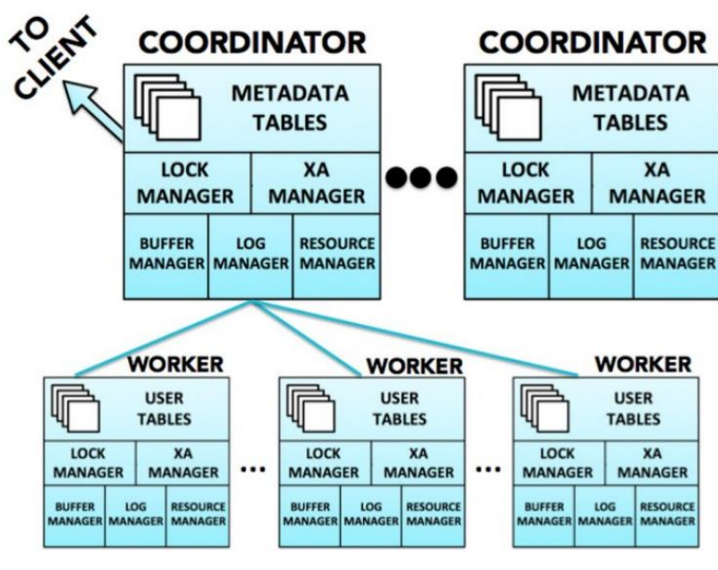
\includegraphics[scale=.7]{images/Component.png}}
\captionsetup{font=Large}
\caption{Kiến trúc hệ thống \cite{arnold2019hrdbms}}
\label{fig:Component}
\end{figure}

Kiến trúc của hệ thống HRDBMS gồm 2 thành phần chính là: worker và coordinator:
Coordinator đảm nhiệm vai trò giao tiếp với người dùng (client), chịu trách nghiệm tối ưu truy vấn. quản lý tài nguyên trên toàn cụm (cluster), phân phối giao dịch (Transaction coordination) đảm bảo tính nhất quán của các giao dịch (transaction).

Worker đảm nhiệm vai trò lưu trữ dữ liệu và thực thi các truy vấn nhận từ Coordinator. 

Quy trình mà giải pháp sẽ cài đặt: Client (người dùng) gửi sql command cho Coordinator. Coordinator sẽ giao tác vụ (task) cho các worker dựa vào dữ liệu mà chúng đang lưu trữ. Worker thực hiện truy vấn mà chúng đang lưu trữ sau khi hoàn thành gửi kết quả truy vấn cho Coordinator. Coordiantor tổng hợp kết quả gữi từ các woker và trả kết quả cuối cùng cho người dùng như hình \ref{fig:diagramworkflow}.

\begin{figure}[htbp]
\centerline{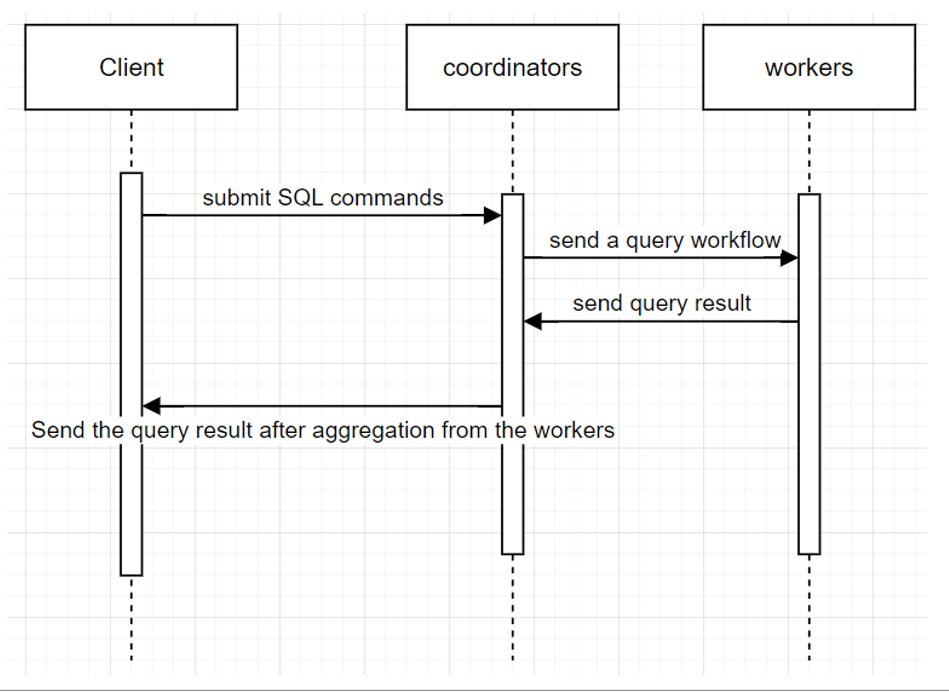
\includegraphics[scale=.7]{images/diagramworkflow.png}}
\captionsetup{font=Large}
\caption{Quy trình tối ưu truy vấn}
\label{fig:diagramworkflow}
\end{figure}

Quy trình này giúp tận dụng sức mạnh của nhiều máy chủ để xử lý dữ liệu và truy vấn một cách song song và hiệu quả hơn.
Quá trình tối ưu truy vấn trong HRDBMS gồm 3 giai đoạn

Giai đoạn 1 Global Optimization như hình \ref{fig:phase1}
“Global Optimization là một giai đoạn trong quá trình tối ưu hóa truy vấn trong hệ thống cơ sở dữ liệu\cite{arnold2019hrdbms}. Trong giai đoạn này, các phép tối ưu hóa sử dụng hai phương pháp: heuristic và cost-based.

Heuristic optimization là phương pháp sử dụng các quy tắc, kinh nghiệm và giải thuật đơn giản để tối ưu hóa truy vấn. Chẳng hạn như, phương pháp đặt bảng nhỏ trước, chọn giá trị được lặp lại ít nhất cho điều kiện WHERE, ...

Cost-based optimization là phương pháp sử dụng các thống kê và mô hình tính toán chi phí để đánh giá và so sánh các kế hoạch truy vấn khác nhau. Nó sẽ lựa chọn kế hoạch truy vấn có chi phí thấp nhất.

Trong giai đoạn này, tối ưu hóa truy vấn sẽ được thực hiện mà không quan tâm đến việc phân phối dữ liệu trên các node trong hệ thống phân tán. Giai đoạn này thường sử dụng trước khi thực hiện phân phối dữ liệu và thực hiện tối ưu hóa cục bộ trên mỗi node trong hệ thống.

“HRDBMS giảm số lần truy cập vào dữ liệu trong các truy vấn lồng nhau (de-correlate and un-nest). Sau đó áp dụng một số biến thể của thuật toán có tên là greedy join enumeration\cite{arnold2019hrdbms}. HRDBMS sử dụng thống kê để ước tính số hàng sẽ được đầu ra bởi mỗi khả năng join. Sau đó, nó sắp xếp các join theo cách cố gắng giảm thiểu tổng số hàng được xử lý bởi mỗi lần join vẫn cho ra kết quả chính xác.

\begin{figure}[htbp]
\centering
\makebox[\linewidth]{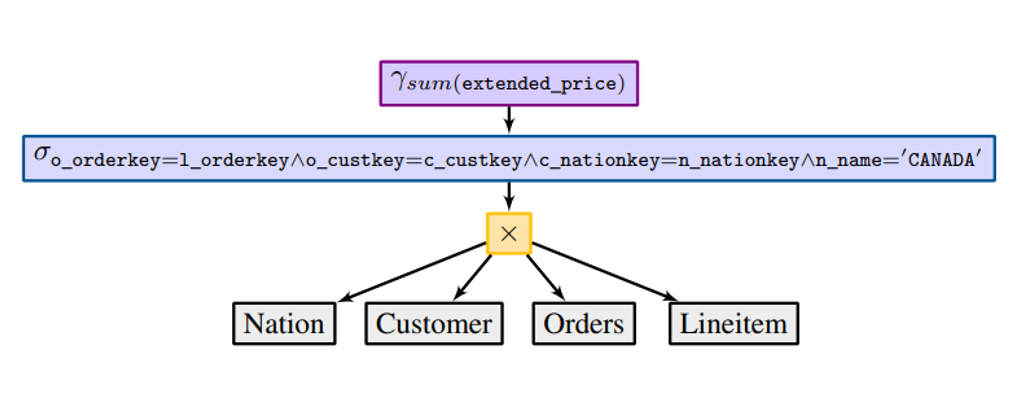
\includegraphics[width=1.3\textwidth,keepaspectratio]{images/phase1.png}}
\captionsetup{font=Large}
\caption{Kế hoạch truy vấn ban đầu \cite{arnold2019hrdbms}}
\label{fig:phase1}
\end{figure}

HRDBMS sử dụng left-deep như hình \ref{fig:phase2}  là một kiểu kế hoạch truy vấn trong hệ thống cơ sở dữ liệu quan hệ. Các bảng được kết nối từ trái sang phải theo thứ tự liên tiếp. như hình bên dưới ta thấy được nation và customer được join đầu tiên sau đó tới orders cuối cùng tới lineitem.

\begin{figure}[htbp]
\centering
\makebox[\linewidth]{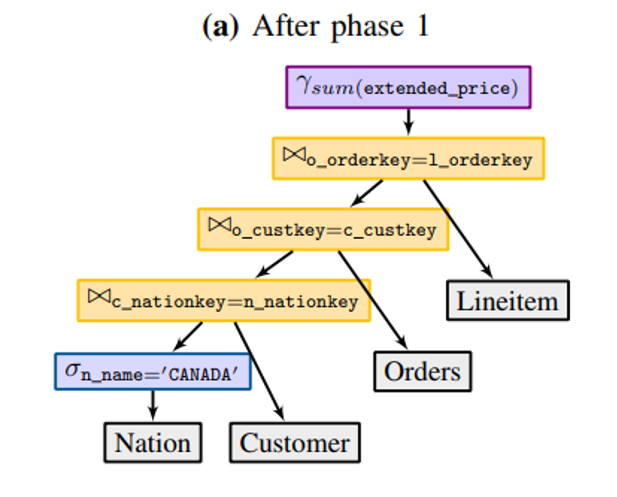
\includegraphics[width=1.3\textwidth,keepaspectratio]{images/phase2.png}}
\captionsetup{font=Large}
\caption{Kế hoạch tối ưu truy vấn của giai đoạn đầu tiên \cite{arnold2019hrdbms}}
\label{fig:phase2}
\end{figure}

Giai đoạn 2 Dataflow Conversion 
“Giai đoạn này là cây toán tử (operator tree) được chuyển thành dòng dữ liệu phân tán(distributed dataflow) đơn giản bằng cách chia mỗi toán tử quét riêng lẻ cho từng phân đoạn(fragment) dựa trên điều kiện truy vấn” \cite{arnold2019hrdbms}. Phân đoạn là một phần của bảng dữ liệu, được chia nhỏ và lưu trữ trên các woker khác nhau trong cụm phân tán việc này giúp xử lý và truy vấn dữ liệu trở nên dễ dàng hơn và hiệu quả hơn như hình \ref{fig:phase3}. 

\begin{figure}[htbp]
\centering
\makebox[\linewidth]{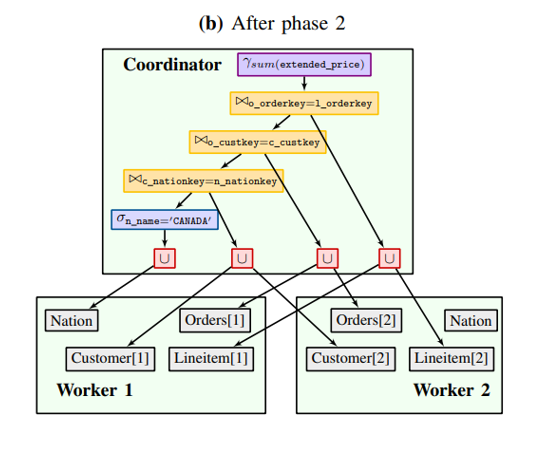
\includegraphics[width=1.3\textwidth,keepaspectratio]{images/phase3.png}}
\captionsetup{font=Large}
\caption{Biểu đồ dòng dữ liệu được tạo ra \cite{arnold2019hrdbms}}
\label{fig:phase3}
\end{figure}

Giai đoạn 3 Dataflow Optimization 
“Trong giai đoạn này sẽ phân chia lại công việc từ Coordiantor sẽ giao cho các Woker” như hình \ref{fig:phase4}. Mục đích của việc này là tận dụng các phân đoạn đã được lưu trong worker để giảm lượng giao tiếp không cần thiết. Việc còn lại của Coordinator là tổng hợp lại kết quả từ các worker gửi về và trả kết quả cho client.


\begin{figure}[htbp]
\centering
\makebox[\linewidth]{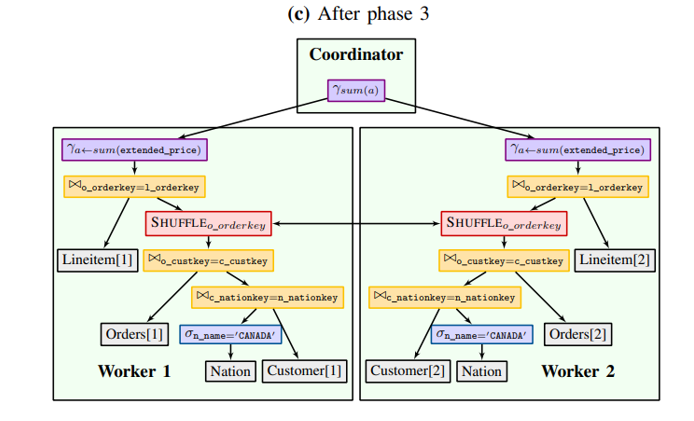
\includegraphics[width=1.3\textwidth,keepaspectratio]{images/phase4.png}}
\captionsetup{font=Large}
\caption{Giai đoạn tối ưu hóa cuối cùng \cite{arnold2019hrdbms}}
\label{fig:phase4}
\end{figure}




Để đánh giá hiệu quả và tiềm năng của giải pháp, luận văn dự kiến sẽ so sánh giải pháp với các cơ sở dữ liệu Apache Hive\footnote{https://hive.apache.org/general/downloads} , Spark SQL\footnote{https://spark.apache.org/downloads.html}, Greenplum\footnote{https://github.com/greenplum-db/gpdb/releases}  độ đo hiệu suất (performance) và khả năng mở rộng (scalability). Cụ thể sẽ sử dụng độ đo TPC-H. TPC-H là một bộ chuẩn kiểm tra hiệu suất (benchmark) cho các hệ thống cơ sở dữ liệu. TPC-H được thiết kế để đánh giá hiệu năng của các hệ thống cơ sở dữ liệu trong việc xử lý các truy vấn phức tạp, chủ yếu liên quan đến các tác vụ OLAP (Online Analytical Processing). TPC-H gồm 22 truy vấn chuẩn và một tập dữ liệu tổng hợp được tạo ra dựa trên mô hình dữ liệu quan hệ với 8 bảng (PART, SUPPLIER, PARTSUPP, CUSTOMER, ORDERS, LINEITEM, NATION, và REGION)\footnote{\url{https://www.tpc.org/TPC_Documents_Current_Versions/pdf/TPC-H_v3.0.1.pdf}}.
Cụ thể để đánh giá hiệu suất của một hệ thống cơ sở dữ liệu thực hiện các bước sau:

\textbf{Tải về và cài đặt TPC-H:} Truy cập trang chủ của TPC-H\footnote{https://www.tpc.org/TPC\_Documents\_Current\_Versions/download\_programs/tools-download-request5.asp} để tải về mã nguồn.

\textbf{Tạo cơ sở dữ liệu:} Trên hệ thống tạo một cơ sở dữ liệu mới để chứa dữ liệu TPC-H.

\textbf{Tạo bảng và khóa ngoại: }Dựa trên định nghĩa của TPC-H, sử dụng lệnh SQL để tạo các bảng (CUSTOMER, SUPPLIER, PART, PARTSUPP, REGION, NATION, ORDERS, LINEITEM)  và khóa ngoại tương ứng.

\textbf{Sinh dữ liệu: }Trong thư mục chứa mã nguồn TPC-H, biên dịch và xây dựng công cụ dbgen theo hướng dẫn. Sử dụng dbgen để sinh dữ liệu mẫu cho các bảng. Thay đổi thông số SF (Scale Factor) để điều chỉnh kích thước dữ liệu.Các tệp dữ liệu được sinh ra sẽ có định dạng “.tbl”.

\textbf{Nạp dữ liệu vào cơ sở dữ liệu: }Import dữ liệu từ các tệp .tbl vào các bảng tương ứng trong cơ sở dữ liệu. 

\textbf{Sinh truy vấn:} Sử dụng qgen để sinh truy vấn mẫu cho TPC-H. Thông tin 22 truy vấn 

\begin{itemize}
\item Truy vấn 1 (Pricing Summary Report Query): Tính toán một báo cáo giá cả tổng hợp cho các dòng sản phẩm trong một khoảng thời gian nhất định.
\item Truy vấn 2 (Minimum Cost Supplier Query): Tìm nhà cung cấp có chi phí nhỏ nhất cho mỗi sản phẩm trong một quốc gia.
\item Truy vấn 3 (Shipping Priority Query): Tìm 10 đơn hàng lớn nhất chưa được giao trong một khoảng thời gian nhất định.
\item Truy vấn 4 (Order Priority Checking Query): Đếm số lượng đơn hàng chưa được giao trong mỗi loại ưu tiên.
\item Truy vấn 5 (Local Supplier Volume Query): Tính tổng giá trị đơn hàng của các nhà cung cấp địa phương trong mỗi quốc gia.
\item Truy vấn 6 (Forecasting Revenue Change Query): Dự đoán doanh thu thay đổi dựa trên việc áp dụng một chiết khấu nhất định cho các đơn hàng trong một khoảng thời gian nhất định.
\item Truy vấn 7 (Volume Shipping Query): Tính tổng giá trị đơn hàng giữa các quốc gia trong một khoảng thời gian nhất định.
\item Truy vấn 8 (National Market Share Query): Tính tổng giá trị đơn hàng của một phân khúc thị trường trong một quốc gia nhất định.

Truy vấn 9 (Product Type Profit Measure Query): Tính lợi nhuận của một loại sản phẩm nhất định trong một khoảng thời gian nhất định.
\item Truy vấn 10 (Returned Item Reporting Query): Báo cáo các mặt hàng bị trả lại trong một khoảng thời gian nhất định.
\item Truy vấn 11 (Important Stock Identification Query): Xác định các sản phẩm quan trọng có tồn kho lớn hơn một giá trị nhất định.
\item Truy vấn 12 (Shipping Modes and Order Priority Query): Đánh giá tỷ lệ các phương thức vận chuyển và mức độ ưu tiên của đơn hàng trong một khoảng thời gian nhất định.
\item Truy vấn 13 (Customer Distribution Query): Đếm số lượng khách hàng có lượng đơn hàng trong một khoảng nhất định.
\item Truy vấn 14 (Promotion Effect Query): Tính tỷ lệ doanh thu khuyến mãi so với tổng doanh thu trong một khoảng thời gian nhất định.
\item Truy vấn 15 (Top Supplier Query): Xác định nhà cung cấp hàng đầu dựa trên tổng giá trị đơn hàng.

\item Truy vấn 16 (Parts/Supplier Relationship Query): Đếm số lượng nhà cung cấp cung cấp các bộ phận phù hợp với điều kiện nhất định.
\item Truy vấn 17 (Small-Quantity-Order Revenue Query): Tính tổng doanh thu cho các đơn hàng có số lượng sản phẩm nhỏ hơn mức trung bình của một loại sản phẩm nhất định.
\item Truy vấn 18 (Large-Volume-Customer Query): Liệt kê các đơn hàng có giá trị lớn hơn một ngưỡng nhất định của những khách hàng mua nhiều.
\item Truy vấn 19 (Discounted Revenue Query): Tính tổng doanh thu cho các đơn hàng có chiết khấu nằm trong một khoảng nhất định và số lượng sản phẩm nằm trong một khoảng nhất định.
\item Truy vấn 20 (Potential Part Promotion Query): Tìm các nhà cung cấp tiềm năng có thể cung cấp các bộ phận phù hợp với điều kiện nhất định trong một chiến dịch khuyến mãi.
\item Truy vấn 21 (Supplier's Unfulfilled Orders Query): Xác định các nhà cung cấp mà tỷ lệ đơn hàng chưa được thực hiện lớn hơn một ngưỡng nhất định.
\item Truy vấn 22 (Global Sales Opportunity Query): Đếm số lượng khách hàng có tổng giá trị đơn hàng nằm trong một khoảng giá trị nhất định.
    
\end{itemize}


\textbf{Chạy các truy vấn TPC-H:} Thực thi lần lượt các truy vấn TPC-H trên hệ thống DBMS. Ghi lại thời gian chạy cho mỗi truy vấn.

\textbf{Tính toán và phân tích kết quả:} So sánh kết quả hiệu năng của hệ thống DBMS với các giá trị tham chiếu từ TPC-H hoặc với kết quả của các hệ thống khác để đánh giá hiệu suất của hệ thống DBMS.

Để đánh giá hiệu suất của hệ thống dự kiến thực hiện trên 8 node sử dụng môi trường AWS(Amazon Web Services) EC2 c5n.9xlarge với 32 vCPU và 96GB RAM trên mỗi node.


\begin{table}[htbp]
\centerline{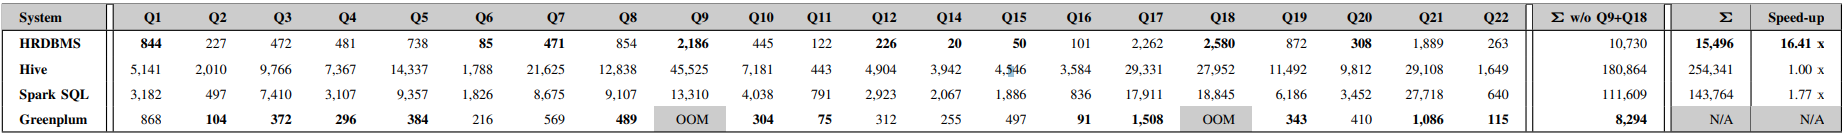
\includegraphics[scale=0.43]{images/test1.png}}
\captionsetup{font=Large}
\caption{Kết quả thực thi trong 8 node \cite{arnold2019hrdbms}}
\label{fig:test1}
\end{table}


Các cột trong bảng:
Q1 - Q22: Thời gian thực thi của các truy vấn TPC-H (được đo bằng mili giây) trên mỗi hệ thống DBMS.

$\Sigma$ w/o Q9+Q18: Tổng thời gian thực thi của tất cả các truy vấn, trừ Q9 và Q18, trên mỗi hệ thống quản lý cơ sở dữ liệu (DBMS).

$\Sigma$: Tổng thời gian thực thi của tất cả các truy vấn trên mỗi hệ thống DBMS.

Speed-up: Chỉ số tăng tốc so với Hive, được tính bằng tổng thời gian thực thi của Hive chia cho tổng thời gian thực thi của mỗi hệ thống DBMS.

Bảng \ref{fig:test1} so sánh hiệu năng này cho thấy sự khác biệt rõ rệt giữa các hệ thống quản lý cơ sở dữ liệu (DBMS) khi thực hiện các truy vấn TPC-H. Dưới đây là đánh giá của mỗi hệ thống dựa trên bảng này:
HRDBMS có hiệu năng xuất sắc so với các hệ thống DBMS khác. Tổng thời gian thực thi của HRDBMS là 15.496 ms, nhanh hơn rất nhiều so với Hive và Spark SQL. Chỉ số tăng tốc của HRDBMS so với Hive là 16,41, cho thấy nó hoạt động nhanh hơn 16,41 lần. HRDBMS thực hiện tốt hơn trong hầu hết các truy vấn và đặc biệt nổi bật trong truy vấn Q9 và Q18.
Hive là hệ thống DBMS chậm nhất trong bảng so sánh này, với tổng thời gian thực thi là 254.341 ms và chỉ số tăng tốc là 1 (được sử dụng làm tiêu chuẩn so sánh). Hive thực hiện chậm nhất trong các truy vấn Q9 và Q18, mất 45.525 ms và 27.952 ms tương ứng.
Spark SQL có hiệu năng tốt hơn Hive nhưng thấp hơn HRDBMS. Tổng thời gian thực thi của Spark SQL là 143.764 ms, và chỉ số tăng tốc so với Hive là 1,77. Spark SQL thực hiện truy vấn Q9 và Q18 với thời gian tương đối nhanh, chỉ mất 13.310 ms và 18.845 ms.
Greenplum có hiệu năng tốt hơn Hive trong một số truy vấn, nhưng không thể hoàn thành truy vấn Q9 do hết bộ nhớ (Out Of Memory - OOM). Do đó, không có số liệu tổng thời gian thực thi và chỉ số tăng tốc cho Greenplum. 

Trên cơ sở bảng \ref{fig:test1} thì HRDBMS là hệ thống DBMS có hiệu năng tốt nhất khi thực hiện các truy vấn TPC-H.

\subsection{Các phương pháp nghiên cứu }
    
Các phương pháp nghiên cứu bao gồm:

\begin{itemize}
\item Xác định vấn đề nghiên cứu: Dựa trên kiến thức lý thuyết về HRDBMS và kết quả phân tích, xác định vấn đề cụ thể, thực tế và có ý nghĩa về quản lý và truy vấn dữ liệu lớn để tập trung nghiên cứu và giải quyết.
\item Chuẩn bị các phần mềm và tập dữ liệu dùng để so sánh: Thực hiện cài đặt và cấu hình các công cụ được sử dụng trong lĩnh vực xử lý và quản lý dữ liệu, nhằm mục đích đối chiếu với HRDBMS gồm Apache Hive, Spark SQL và Greenplum. Sử dụng các tập dữ liệu tổng hợp từ TPC-H làm tiêu chuẩn để đánh giá và so sánh.
\item Thiết lập môi trường thử nghiệm trên các dịch vụ đám mây: Đăng ký và sử dụng các dịch vụ đám mây như Amazon Web Services (AWS) và Google Cloud Platform (GCP) để triển khai và thiết lập môi trường thử nghiệm, bao gồm việc cài đặt và cấu hình các máy chủ ảo, cơ sở dữ liệu HRDBMS và các dịch vụ liên quan khác.
\item Biên dịch, sửa đổi và chạy mã nguồn HRDBMS: Tiến hành biên dịch, sửa đổi và chạy mã nguồn trên môi trường phù hợp.
\item Đề xuất giải pháp và phương pháp giải quyết: Đưa ra các giải pháp và phương pháp giải quyết vấn đề nghiên cứu, bao gồm cải tiến thuật toán, tối ưu hóa hiệu suất, độ tin cậy, khả năng mở rộng, vv. của HRDBMS.
\item Thực nghiệm và kiểm chứng: Thiết kế và triển khai các mô phỏng để kiểm chứng tính hiệu quả, độ tin cậy và khả năng mở rộng của các giải pháp đề xuất cho HRDBMS. Thu thập, phân tích và đánh giá kết quả thực nghiệm để rút ra nhận xét.
\item Viết tài liệu hướng dẫn cài đặt và vận hành giải pháp HRDBMS.
\item Viết luận văn tổng kết lại toàn bộ quá trình và kết quả của việc áp dụng HRDBMS
\end{itemize}


\subsection{Nội dung và phạm vi của vấn đề sẽ đi sâu nghiên cứu}
\begin{itemize}
\item Bản luận văn hoàn chỉnh, mô tả chi tiết cơ sở lý thuyết và các kết quả thu được từ việc nghiên cứu và áp dụng HRDBMS. Luận văn sẽ bao gồm phân tích, đánh giá và đề xuất các giải pháp mới để cải thiện hiệu suất, độ tin cậy và khả năng mở rộng của hệ thống quản lý cơ sở dữ liệu phân tán.
\item Mã nguồn của HRDBMS đã được phát triển và tối ưu hóa một cách đáng kể. Mã nguồn này sẽ đảm bảo tính ổn định, hiệu năng cao và khả năng mở rộng tốt của hệ thống khi xử lý các tác vụ quản lý dữ liệu lớn.
\item Dữ liệu từ TPC-H được chỉnh sửa để phục vụ cho việc đánh giá, thử nghiệm và so sánh hiệu suất của các giải pháp đề xuất. Điều này có thể bao gồm việc tạo ra các tập dữ liệu mô phỏng hoặc sử dụng các tập dữ liệu thực tế từ các nguồn như TPC-H.
\item Các tài liệu kỹ thuật hướng dẫn chi tiết về phương pháp tái tạo các sản phẩm nghiên cứu, bao gồm hướng dẫn sử dụng giải pháp HRDBMS được phát triển, phương pháp tiếp cận và triển khai các giải pháp đề xuất trong thực tế, cũng như hướng dẫn cho các nghiên cứu sau này liên quan đến đề tài.
\end{itemize}

\subsection{Nơi thực hiện đề tài nghiên cứu của luận văn}
Khoa Công nghệ thông tin – Trường đại học Khoa học Tự Nhiên – Đại học quốc gia TP.Hồ Chí Minh
    
\subsection{Thời gian thực hiện}

\begin{longtable}{|>{\raggedright\arraybackslash}p{4cm}|>{\raggedright\arraybackslash}p{3cm}|>{\raggedright\arraybackslash}p{3cm}|>{\raggedright\arraybackslash}p{5cm}|}
\hline
\textbf{Công việc} & \textbf{Thời gian bắt đầu} & \textbf{Thời gian kết thúc} & \textbf{Mô tả} \\
\hline
Nghiên cứu lý thuyết và định hướng đề tài & 01/06/2023 & 15/06/2023 & Trong giai đoạn này, sẽ tập trung vào việc đọc và hiểu lý thuyết về HRDBMS và các công nghệ liên quan. Đồng thời, xác định rõ hướng đi cho đề tài. \\
\hline
Chuẩn bị và tìm hiểu các công cụ và dữ liệu cho việc so sánh & 16/06/2023 & 30/06/2023 & Thực hiện cài đặt và cấu hình các công cụ được sử dụng trong lĩnh vực xử lý và quản lý dữ liệu, nhằm mục đích đối chiếu với HRDBMS gồm Apache Hive, Spark SQL và Greenplum và sử dụng các tập dữ liệu tổng hợp từ TPC-H làm tiêu chuẩn để đánh giá và so sánh. \\
\hline
Thiết lập môi trường thử nghiệm & 01/07/2023 & 15/07/2023 & Đăng ký và sử dụng các dịch vụ đám mây như Amazon Web Services (AWS) và Google Cloud Platform (GCP) để triển khai và thiết lập môi trường thử nghiệm, bao gồm việc cài đặt và cấu hình các máy chủ ảo, cơ sở dữ liệu và các dịch vụ liên quan khác. \\
\hline
Chỉnh sửa và vận hành mã nguồn HRDBMS & 01/08/2023 & 31/08/2023 & Tiến hành biên dịch, sửa đổi và chạy mã nguồn trên môi trường phù hợp. \\
\hline
Đưa ra giải pháp và phương pháp giải quyết vấn đề & 01/09/2023 & 30/09/2023 & Đưa ra các giải pháp và phương pháp giải quyết vấn đề nghiên cứu, bao gồm cải tiến thuật toán, tối ưu hóa hiệu suất, độ tin cậy, khả năng mở rộng, vv. \\
\hline
Tiến hành thử nghiệm và đánh giá kết quả & 01/10/2023 & 31/10/2023 & Thiết kế và triển khai các mô phỏng để kiểm chứng tính hiệu quả, độ tin cậy và khả năng mở rộng của các giải pháp đề xuất. Thu thập, phân tích và đánh giá kết quả thực nghiệm \\
\hline
Soạn thảo, chỉnh sửa và hoàn thiện luận văn & 01/11/2023 & 01/12/2023 & Tập trung vào việc viết và chỉnh sửa bản luận văn, mô tả chi tiết cơ sở lý thuyết và các kết quả thu được từ nghiên cứu, bao gồm phân tích, đánh giá và đề xuất các giải pháp mới cho hệ thống. \\
\hline
\end{longtable}

    
    
    
    \pagebreak 
    %TÀI LIỆU TRÍCH DẪN
    %Đây là ví dụ
    \bibliographystyle{ieeetr}
    \bibliography{References/references}
    \nocite{*}

    \begin{table}[h]
    \centering
        \begin{tabular}{p{7cm}p{7cm}}
        \textbf{\begin{tabular}[c]{@{}c@{}}\\XÁC NHẬN\\CỦA NGƯỜI HƯỚNG DẪN\\ \textit{(Ký và ghi rõ họ tên)}\end{tabular}} & \textbf{\begin{tabular}[c]{@{}c@{}}\textit{TP. Hồ Chí Minh, ngày... tháng... năm...}\\HỌC VIÊN THỰC HIỆN\\\textit{(Ký và ghi rõ họ tên}) \end{tabular}}
        \end{tabular}
    \end{table}
    
\end{document}


